\section{Virtual Honeypot}
A virtual honeypot is a software that emulates a vulnerable system or network to attract intruders and study their behavior, It is easy to implement and unlike hardware-based, it can contain in a single Virtual machine  multiple honeypots implemented for different purposes and since it is all emulated it does not allow infiltrations from the outside that can use the same virtual honeypot to attack the system, but  because it is completely emulated, a skilled hacker can see the difference from the real system.
\subsection{A tool for virtual honeypot: Honeyd}
Honeyd is a small daemon that creates virtual hosts on a network. It creates low-interaction honeypots thats emulates service of a real OS.
It allows you to create multiple virtual honeypots (each with a different ip) by sharing the resources of the same server.\\
The server via TCP / IP protocol, based on the destination IP address, chooses which honeypot to serve.\\
It only supports TCP, UDP and ICMP protocols.\\
Honeyd ,as eplained in the article \cite{Provos2003HoneydA} is designed for Unix systems and (as the other low-interaction honeypot) it has no OS installed, it has the advantage of run several different operating systems at the same time, each ip has his port to make the service listen and return different fake message returning them to the hacker, this fake message are generated by personality engine to make it look good and logical according to the template.\\
The template is a virtual machine where we can set which port are open, which OS is running etc. each port can be set to be open with a script running on it to simulate the service.\\
\begin{figure}[h!]
  \centering
  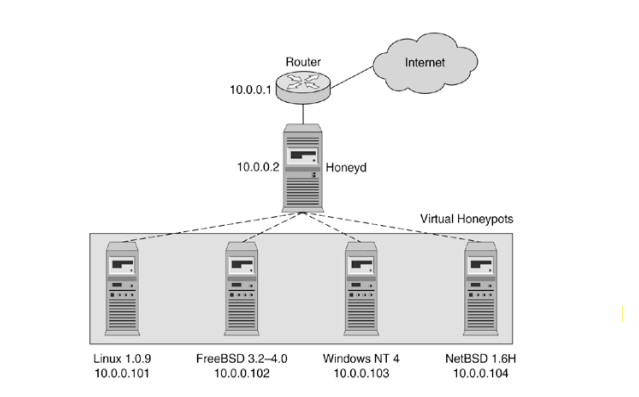
\includegraphics{images/honeyd1.png}
  \caption{Structure of the honeyd}
  \label{fig:irradiances}
\end{figure}
\FloatBarrier
The file Honeyd.conf contains the configuration for the virtual network .\\
Once the template is fixed we can set the IP addresses, at the end we create a network that seems real for the attacker.\\

As soon as a packet arrives, the dispatcher checks that the IP is valid in the configuration file, in the absence of the IP a default model is sent back.
\begin{figure}[h!]
  \centering
  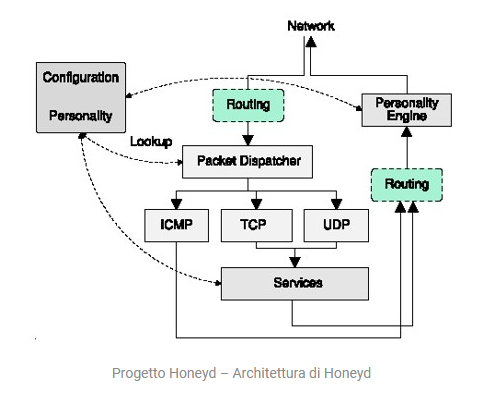
\includegraphics{images/honeyd.png}
  \caption{Implementation of  honeyd}
  \label{fig:irradiances}
\end{figure}
\FloatBarrier
Upon receipt of a request, the framework checks whether the packet concerns an already established connection and in this case forwards it to the corresponding service, otherwise a new process is created for its execution. In addition to local services, a connection redirection mechanism is supported through which it is possible to route a service request to a real system.
Personality engine and configuration engine works together to decide the protocol for transferring according to the configuration (transport and link layer), so before returning the packets to the network, the personality engine modifies the headers to make them compatible with the stack used in the machine's SO.\\
Since attackers often use tools to scan the network and know the operating system running on the system, by default Honeyd uses Nmap's fingerprinting database as a reference for TCP headers and Xprobe's for ICMP headers. In this way he tries to deceive the attackers with their own weapons.
Since both the DOS Honeypot and Malware Honeypot works with TCP/IP protocol, we think it should be a good idea to run this daemon inside one Raspberry Pi and generate both the honeypots in virtual.
Honeyd is a very interesting low interaction honeypot but its problem is its age, apparently the project is outdated and nobody seems to upgrade it.\\
Another problem given by age is that hacker tools are evolving during time so identifying this honeypot is not so hard.\\
Now with a basic scan it is possible to find which ports are open, connect to them and as soon as the connection is established the hacker (based on the response the honeyd provide) understand quickly that something is wrong and abort the attack.

